\newpage
\section{Proposed Layout}

\begin{figure}
  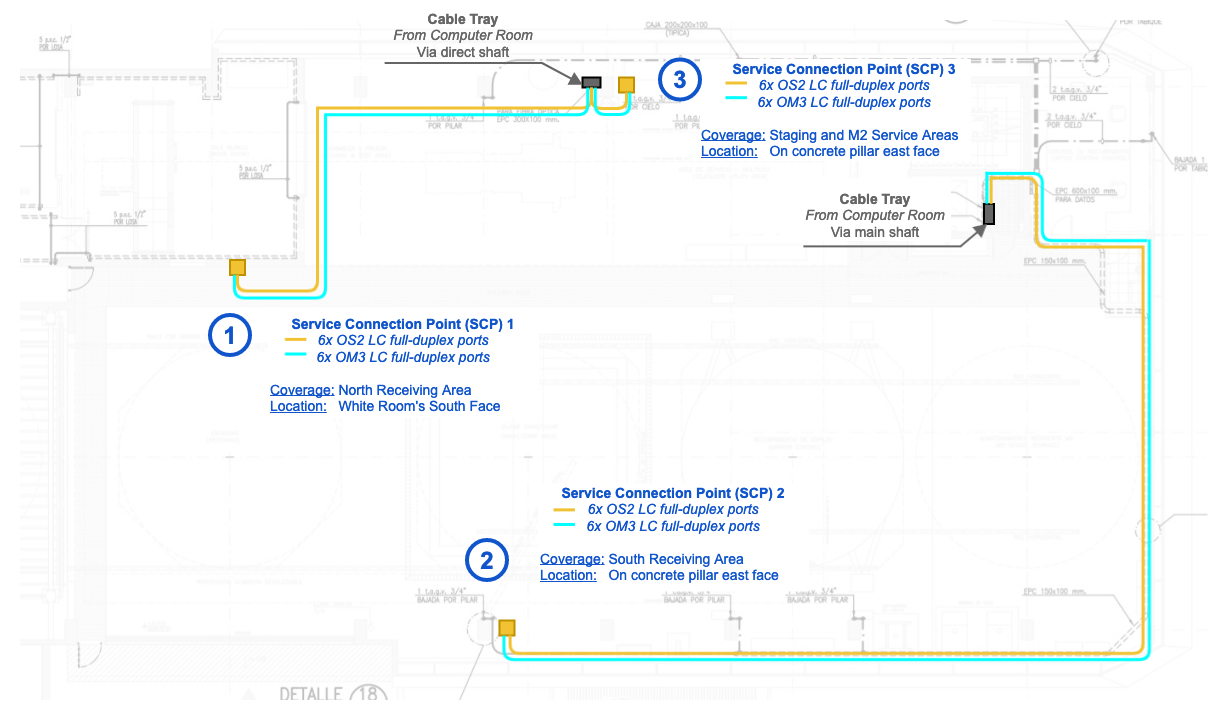
\includegraphics[width=16cm]{images/image-001.png}
  \centering
  \caption{Proposed layout}
\end{figure}

\subsection{Explanation}

As the images describe, it is possible to watch the proposed location of the SCP around the laboratories on the third floor, where each cabinet will contain inside a PDU, UPS, and a Gigabit Switch.
Also, it will be possible to move at least a few meters the rack from the SCP, with fiber and power extension rolled on a reel assembly

\newpage
\section{Network configuration}
  \subsection{High Level Topology}
  \begin{figure}
    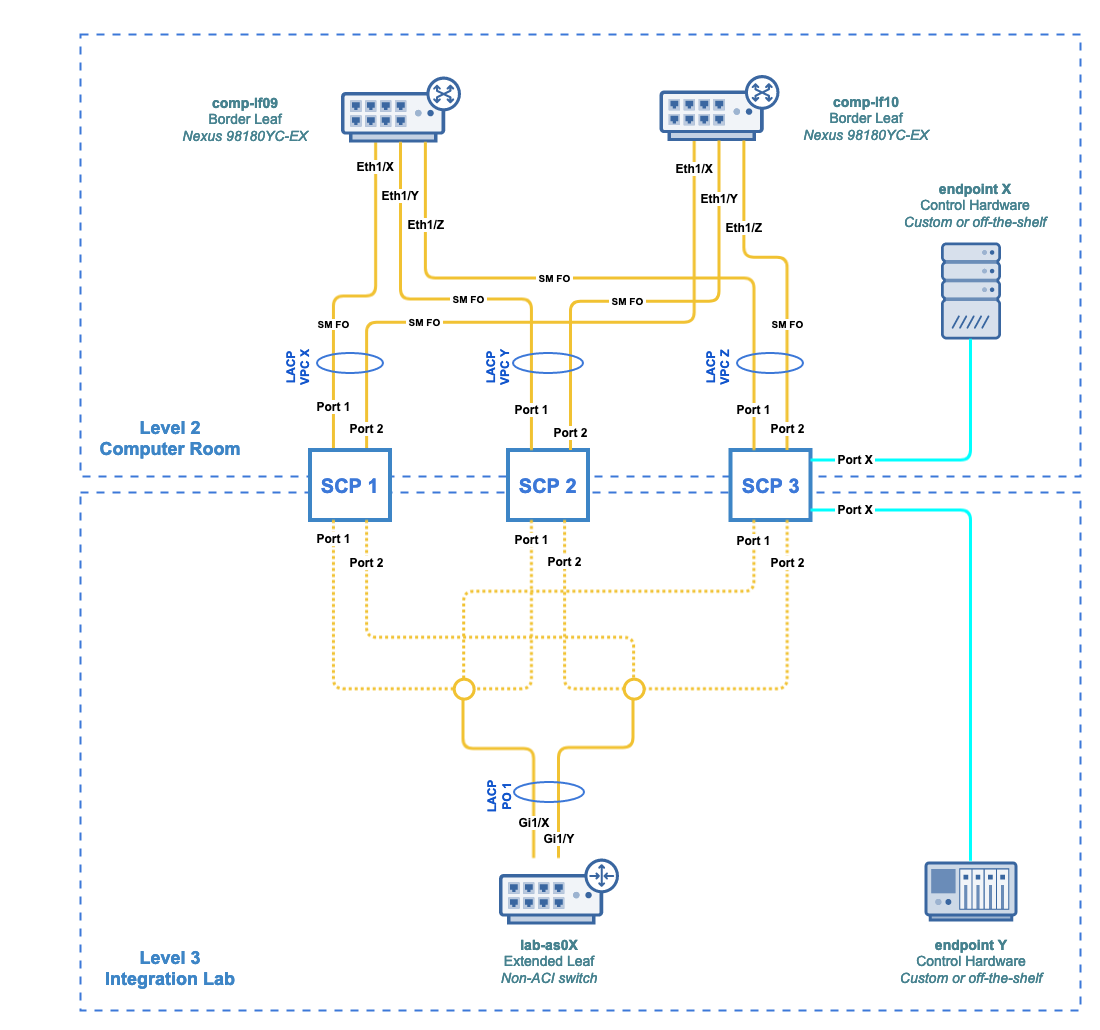
\includegraphics[width=14cm]{images/image-002.png}
    \centering
    \caption{Network configuration High level topology}
  \end{figure}

  \newpage
  \subsection{Explanation}
  The above diagram represents the concept of the "always-on" connections to be implemented. 
  The idea is to have a pair of interfaces in the ACI border leafs pre-configured and always cabled up for this purpose. Each pair of interfaces connects to the Service Connection Points (SCP) so that the switches used for integration at Level 3 can physically roam around the floor. The engineers working in the area can get the connection back online only by moving the fibers to the same ports in the next SCP. 
  The diagram shows only one switch, but there will install a Kit ( i.e., Mobile Rack, Gigabit Switch, UPS, PDU, and Reel assembly) per SCP.
  For network connections, you will want to use single-mode all the time to future-proof the install in case of special integration requirements that ask for more bandwidth.

    Some relevant points to have in consideration for the implementation:
    \begin{itemize}
      \item All vPCs on the datacenter side should be configured in the same way for this to work correctly and without IT intervention.  
      \item The fabric will see the endpoints mac-addresses "flapping" from one port to another, and Syslog may alert about this 
      \item Label everything properly and provide the non-IT engineers with specific instructions for moving a switch from one SCP to another.    \end{itemize}



